\section{Architecture}
\begin{frame}
    \frametitle{Initial approaches}
    \begin{columns}[t]
        \begin{column}{.3\textwidth}
            Predict \emph{exact} words?
            \begin{itemize}
                \item Image CNN + Text transformer
                \item \emph{Twice} the compute of ResNet-50
                \item Learns quite slowly
            \end{itemize}
            \pause
            Bottom line: \underline{Doesn't scale!}
        \end{column}
        \pause
        \begin{column}{.25\textwidth}
            Predict \emph{bag} of words?
            \begin{itemize}
                \item More efficient than exact words
                \item Still difficult due to wide variety of descriptions
            \end{itemize}
        \end{column}
        \pause
        \begin{column}{.45\textwidth}
            \emph{Contrastive} bag of words!
            \begin{itemize}
                \item Contrastive models have been found to learn better representations
                \item More compute-efficient
            \end{itemize}
            \pause

            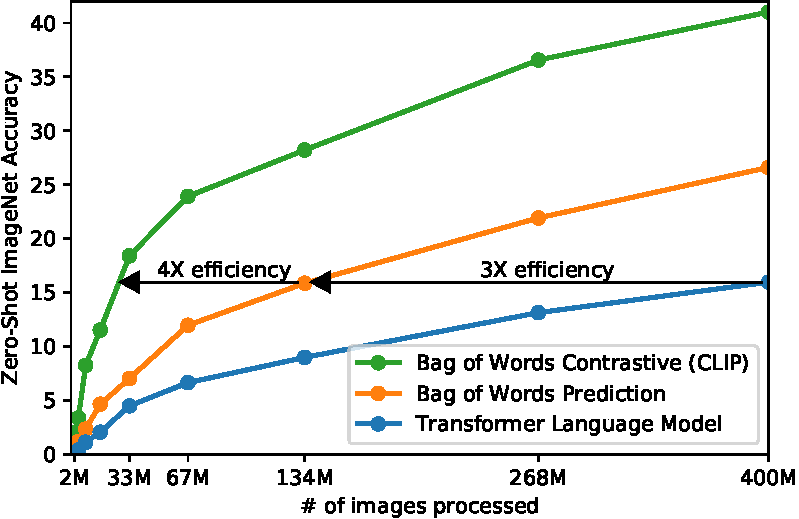
\includegraphics[width=\textwidth]{./images/efficiency-ablation}\framecite{clip}
        \end{column}
    \end{columns}
\end{frame}

\begin{frame}
    \begin{figure}
        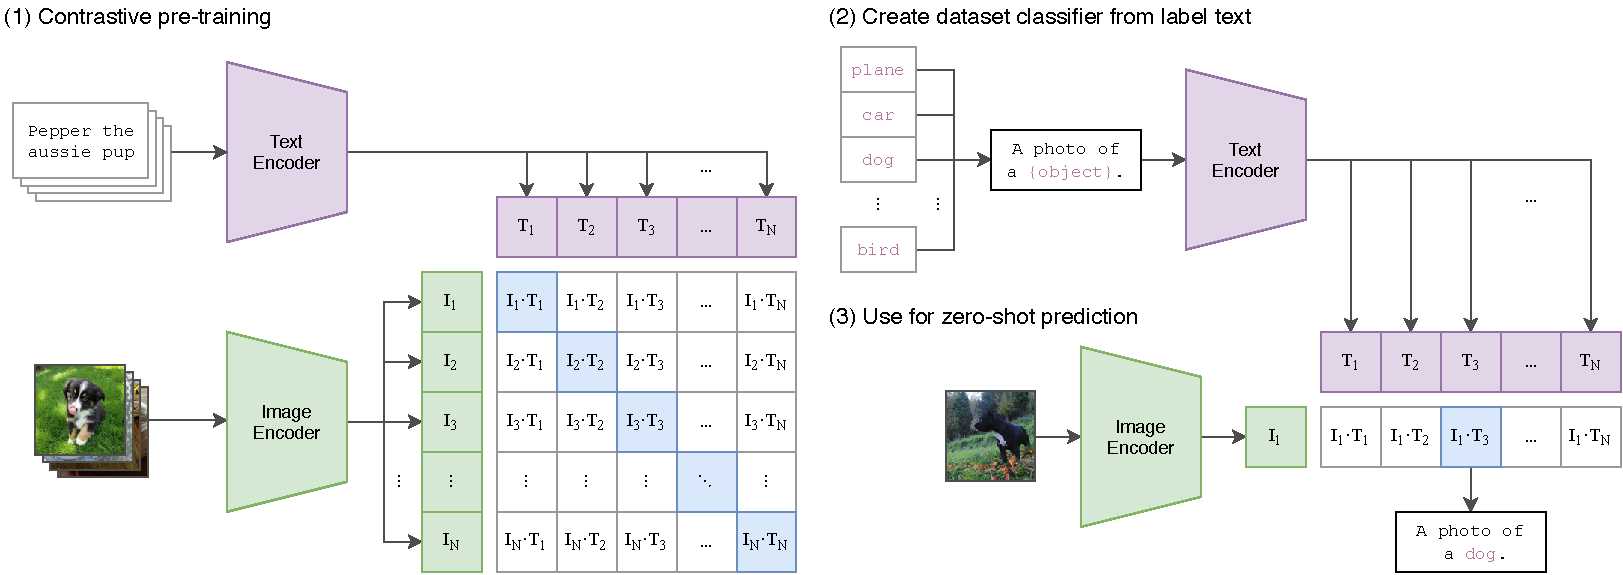
\includegraphics[width=.6\textwidth,trim={0 0 13.5cm 0},clip]{./images/main-diagrams}
        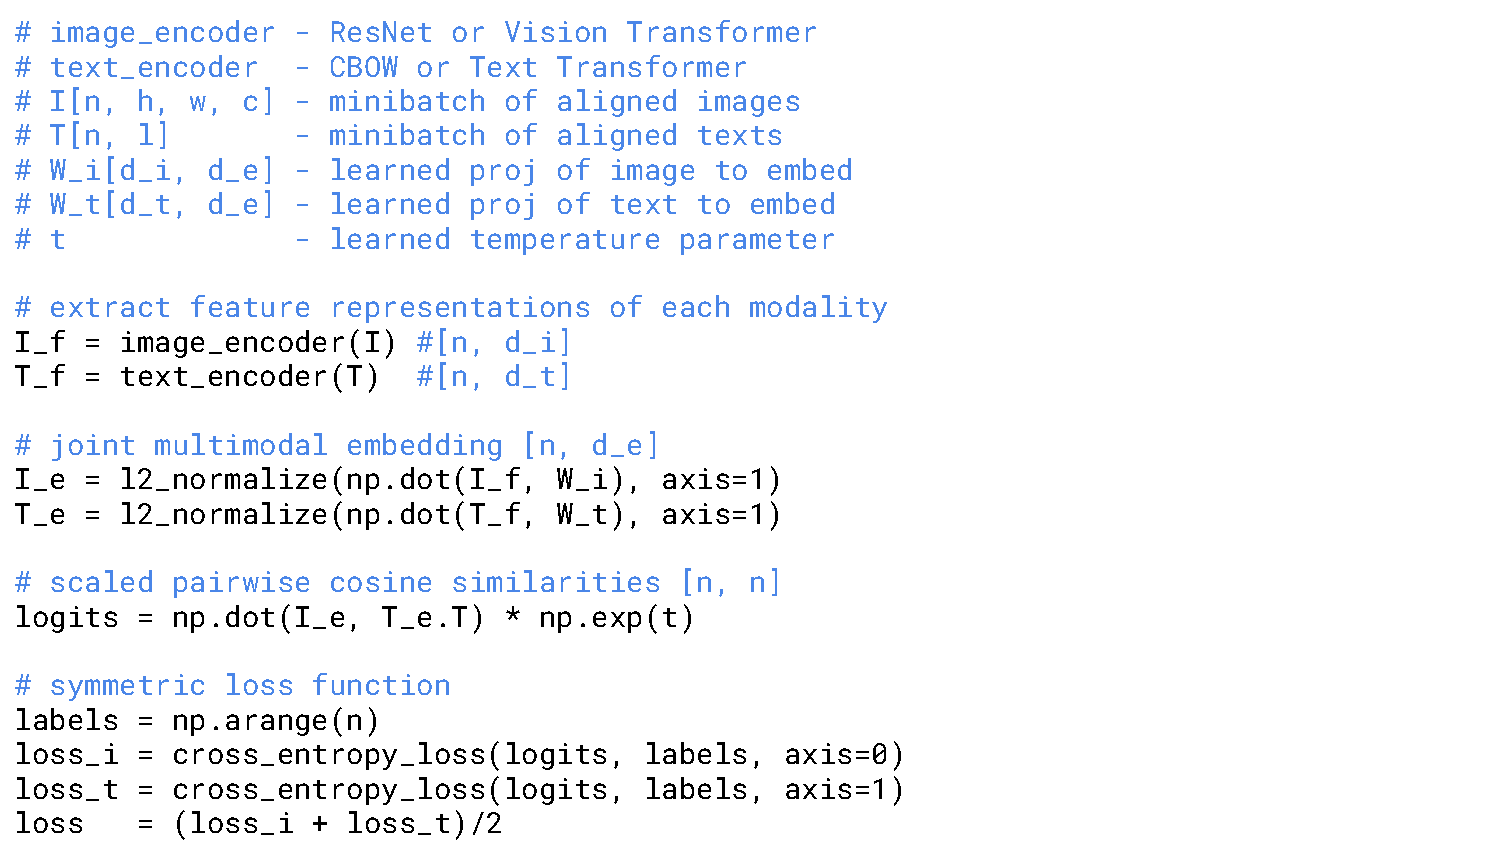
\includegraphics[width=.35\textwidth]{./images/pseudocode}\footfullcite{clip}
    \end{figure}
\end{frame}

\begin{frame}
    \centering
    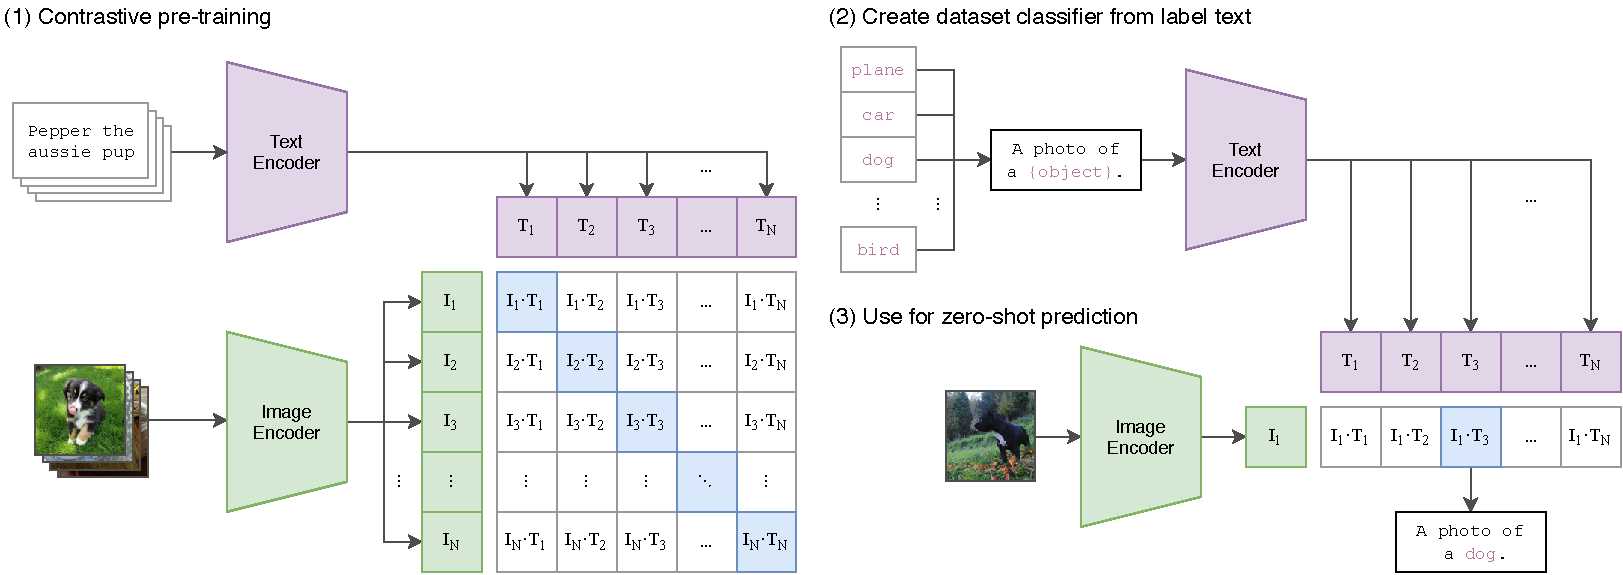
\includegraphics[height=6.5cm,trim={13.5cm 0 0 0},clip]{./images/main-diagrams}\footfullcite{clip}
\end{frame}

% \begin{frame}
%     \frametitle{Underlying Models}
%     \begin{columns}[t]
%         \begin{column}{0.4\textwidth}
%             Text Encoder
%             \begin{itemize}
%                 \item<1-> Transformer
%                 \item<2-> Capacity doesn't affect performance
%             \end{itemize}
%         \end{column}
%         \begin{column}{0.6\textwidth}
%             Image Encoder
%             \begin{itemize}
%                 \item<3-> ResNet with attention layer
%                       \begin{itemize}
%                           \item ResNet-50
%                           \item ResNet-101
%                           \item RN50x4
%                           \item RN50x16
%                           \item<4-> RN50x64: Trained 18 days on 592 V100 GPUs!
%                       \end{itemize}
%                 \item<5-> Vision Transformer
%                       \begin{itemize}
%                           \item ViT-B/16
%                           \item ViT-B/32
%                           \item ViT-L/14: Trained 12 days on 256 V100s
%                           \item<6-> ViT-L/14@336px: Higher resolution,  trained one more epoch. \underline{Performs best!}
%                       \end{itemize}
%             \end{itemize}

%         \end{column}
%     \end{columns}
% \end{frame}

\begin{frame}
    \frametitle{The Dataset}

    \begin{columns}[t]
        \begin{column}{0.5\textwidth}
            Existing datasets
            \begin{itemize}
                \item Crowd-labeled datasets: "only" \~{} 100k images
                \item Large datasets (YFCC100M): Generated filenames, sparse metdata
            \end{itemize}
        \end{column}
        \pause
        \begin{column}{0.5\textwidth}
            Custom dataset: WebImageText (WIT)
            \begin{itemize}
                \item 400 million publicly available image-text pairs
                \item Wide variety: 500.000 different queries, each up to 20.000 image-text pairs
                \item Total word count similar to GPT-2's training data
            \end{itemize}
        \end{column}
    \end{columns}
\end{frame}
